\section{Przetwarzanie danych}\label{sec:przetwarzanie_danych}
\subsection{Zbiór początkowy}\label{subsec:filtrowanie_danych}
Biblioteka \textit{pandas}\cite{mckinney-proc-scipy-2010} została użyta do wczytania danych z pliku \textit{csv} do obiektu \textit{DataFrame}.
Umożliwia ona łatwe i szybkie przetwarzanie danych, a także wygodne operacje na nich. Plik z danymi nie zawiera nagłówków, więc zostały one dodane ręcznie.
zmienna \textit{HEADERS} zawiera listę nazw kolumn, w kolejności odpowiadającej kolejności kolumn w pliku z danymi. Pierwsza kolumna \textit{lettr} jest etykietą klasy, a pozostałe to cechy.
\begin{minted}[linenos,autogobble,frame=lines,framesep=2mm]{python}
import pandas as pd

DATA_PATH = "letter-recognition.data"
HEADERS = [
    "lettr",
    "x-box",
    "y-box",
    "width",
    "high",
    "onpix",
    "x-bar",
    "y-bar",
    "x2bar",
    "y2bar",
    "xybar",
    "x2ybr",
    "xy2br",
    "x-ege",
    "xegvy",
    "y-ege",
    "yegvx",
]
data = pd.read_csv(DATA_PATH, header=None, names=HEADERS)
\end{minted}
\begin{figure}
    \centering
    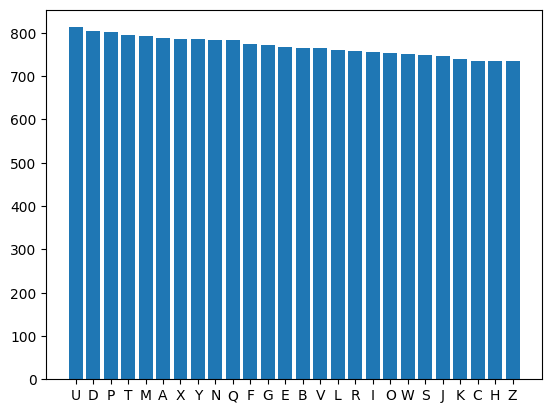
\includegraphics[width=0.5\textwidth]{img/bar_letter_count_initial.png}
    \caption{Początkowy rozkład klas w zbiorze danych.}
    \label{fig:bar_letter_count_initial}
\end{figure}